\documentclass[10pt]{beamer}

% ---------- Theme (PKU dark red, miniframes header) ----------
\useoutertheme[subsection=false]{miniframes}
\useinnertheme{rounded}
\usepackage{amsmath,amssymb,booktabs,graphicx,multirow}
\usepackage{appendixnumberbeamer}

\definecolor{pkured}{RGB}{139,0,0}
\definecolor{pkudark}{RGB}{110,0,0}
\definecolor{blockbg}{RGB}{238,234,234}

\setbeamercolor{structure}{fg=pkured}
\setbeamercolor{section in head/foot}{bg=pkudark,fg=white}
\setbeamercolor{frametitle}{bg=pkured,fg=white}
\setbeamercolor{framesubtitle}{fg=white!85!pkured}
\setbeamercolor{title}{bg=pkured,fg=white}
\setbeamercolor{subtitle}{fg=white}
\setbeamercolor{block title}{bg=pkured,fg=white}
\setbeamercolor{block body}{bg=blockbg,fg=black}
\setbeamercolor{block title alerted}{bg=pkured,fg=white}
\setbeamercolor{block body alerted}{bg=blockbg,fg=black}
\setbeamercolor{alerted text}{fg=red!85!black}
\setbeamercolor{item projected}{bg=pkured,fg=white}

\setbeamertemplate{blocks}[rounded][shadow=true]
\setbeamertemplate{title page}[default][colsep=-4bp,rounded=true,shadow=true]
\setbeamertemplate{items}[ball]
\setbeamertemplate{enumerate items}[ball]
\setbeamertemplate{navigation symbols}{}
\setbeamertemplate{caption}[numbered]
\setbeamerfont{caption}{size=\footnotesize}
\setbeamertemplate{footline}{%
  \hfill\usebeamercolor[fg]{normal text}\scriptsize\insertframenumber\,/\,\inserttotalframenumber\hspace*{3mm}\vspace*{2.5mm}}

\newcommand{\E}{\mathbb{E}}

% ---------- Title ----------
\title{Engineering Enrollment and Wages}
\subtitle{Full-Information Estimation of the Ryoo--Rosen Model}
\author{Max Cheong}
\institute{\small Guanghua School of Management, Peking University}
\date{October 2026\\[2ex]{\scriptsize Code \& data: \href{https://github.com/maxmaxmaxmaxmaxmax373/ryoo-rosen-mle}{\texttt{github.com/maxmaxmaxmaxmaxmax373/ryoo-rosen-mle}}}}

\begin{document}

\begin{frame}[plain]
  \titlepage
\end{frame}

\begin{frame}{Outline}
  \tableofcontents
\end{frame}

% =====================================================
\section[Motivation]{Motivation and Contribution}

\begin{frame}{Booms and Busts in the Market for Engineers}
  \begin{itemize}
    \item \textbf{Large swings:} engineering's share of all bachelor's degrees was 4.2\% in 1976, \alert{7.8\%} in 1985, and 4.7\% in 2000.
    \item \textbf{Wages moved first:} engineers' median earnings relative to all college graduates rose from \alert{1.33 to 1.50} (1972--1982).
    \item \textbf{Recurring debates:} talk of an engineer ``shortage'' in the 1950s (Arrow \& Capron 1959); declining interest again around 1990.
  \end{itemize}
  \vspace{0.3cm}
  \begin{block}{Two Questions}
    \begin{enumerate}
      \item What drives the booms and busts in the market for engineers?
      \item How far do students base their choice of major on the wages they \emph{expect} to earn?
    \end{enumerate}
  \end{block}
  \vspace{0.2cm}
  {\small Students choose a field \textbf{four years} before entering the labor market and are paid over a \textbf{career}: enrollment depends on wage sensitivity \emph{and} on expectations.}
\end{frame}

\begin{frame}{Literature and Contribution}
  \begin{columns}[T]
    \begin{column}{0.47\textwidth}
      \begin{block}{Literature}
        \small
        \begin{itemize}
          \item \textbf{Cobweb:} Freeman (1971, 1975, 1976).
          \item \textbf{Rational expectations:} Siow (1984); Zarkin (1985).
          \item \textbf{Ryoo \& Rosen (2004):} equation by equation, 1950--1990; demand elasticity 1.2--2.2, entry elasticity 2.5--4.5.
          \item \textbf{FIML method:} Hansen \& Sargent (1980, 2013); Sargent (1989).
        \end{itemize}
      \end{block}
    \end{column}
    \begin{column}{0.50\textwidth}
      \begin{block}{This Paper}
        \small
        \begin{enumerate}
          \item Equilibrium solves a \alert{linear-quadratic planning problem}.
          \item Full-information ML with the \alert{Kalman filter}, CPS \& NSF data, 1968--2010.
          \item Career value is a function of the state, not measured or instrumented.
          \item Measurement error, cyclical AR(2) shocks, profile-likelihood intervals.
          \item Rational vs.\ cobweb expectations in \alert{one likelihood}.
        \end{enumerate}
      \end{block}
    \end{column}
  \end{columns}
  \vspace{0.1cm}
  {\small \textbf{Cost of joint estimation:} misspecification in any one equation affects all estimates.}
\end{frame}

\begin{frame}{Preview of Findings}
  \begin{enumerate}
    \item \textbf{Enrollment is highly sensitive to persistent wages.}\\
      A permanent 1\% rise in the relative wage eventually raises the entry share by \alert{$\approx 6\%$} (RE) and $\approx 5\%$ (cobweb).
    \vspace{0.2cm}
    \item \textbf{Swings come from preferences, not wages.}\\
      \alert{97\%} of degree-share variance comes from the attractiveness of engineering, a damped cycle of $\approx$ \alert{22 years}; the observed stock is mostly measurement error.
    \vspace{0.2cm}
    \item \textbf{Expectations cannot be pinned down.}\\
      A cobweb model fits about as well and better matches the comovement of wages and future degrees, but only with a nearly flat demand curve: demand elasticity \alert{1.6 (RE) vs.\ 6.0 (cobweb)}.
  \end{enumerate}
\end{frame}

% =====================================================
\section{Model}

\begin{frame}{Model: Setup and Shocks}
  \begin{itemize}
    \item Annual periods. All variables are \textbf{log ratios} of engineers to all college graduates, in deviations from trend:
      \begin{itemize}
        \item $w_t$: relative wage;\quad $N_t$: relative stock;\quad $n_t$: enrollment share.
        \item Training takes four years: degree share $\pi_t = n_{t-4}$.
      \end{itemize}
    \item Representative firm and household, both wage takers.
    \item Two shocks, each an \textbf{unrestricted AR(2)}:
  \end{itemize}
  \begin{align*}
    \theta_{t+1} &= a_1^\theta\theta_t + a_2^\theta\theta_{t-1} + \sigma_\theta\varepsilon^\theta_{t+1} \quad \text{(demand)}\\
    \psi_{t+1} &= a_1^\psi\psi_t + a_2^\psi\psi_{t-1} + \sigma_\psi\varepsilon^\psi_{t+1} \quad \text{(preference)}
  \end{align*}
  \begin{itemize}
    \item If $a_1^2+4a_2<0$: complex roots $re^{\pm i\omega}$ $\Rightarrow$ \alert{damped cycle} of period $2\pi/\omega$, decay rate $r=\sqrt{-a_2}$.
    \item Discount factor fixed at $\beta=0.96$.
  \end{itemize}
\end{frame}

\begin{frame}{Firms and the Stock of Engineers}
  \small
  \begin{block}{The Firm}
    \[
      \max_{\{N^d_t\}}\; \E_0\sum_{t=0}^{\infty}\beta^t\Big[(f_1+\theta_t)N^d_t-\tfrac{f_2}{2}(N^d_t)^2-w_tN^d_t\Big]
      \;\Longrightarrow\;
      \boxed{w_t=-f_2N^d_t+\theta_t}
    \]
    Static problem; in logs, $1/f_2$ is the \alert{elasticity of demand}.
  \end{block}
  \vspace{0.05cm}
  \begin{block}{The Stock}
    $L_{t+1}=\delta L_t+S_{t-3}$; log-linearize around balanced growth $g$ and difference out all graduates:
    \[
      \boxed{N_{t+1}=\lambda N_t+(1-\lambda)\,n_{t-3}},\qquad \lambda=\frac{\delta}{1+g}.
    \]
    $\lambda$ = share of incumbents in next year's stock; each cohort is small, so the stock \alert{adjusts slowly}.
  \end{block}
\end{frame}

\begin{frame}{Households: Enrollment and Career Value}
  \begin{block}{The Household}
    \[
      \max_{\{n_t\}}\;\E_0\sum_{t=0}^\infty\beta^t\Big[w_tN^h_t-\tfrac{d}{2}n_t^2+d\,\psi_t n_t\Big]
      \quad\text{s.t.}\quad N^h_{t+1}=\lambda N^h_t+(1-\lambda)n_{t-3}
    \]
    \[
      \Longrightarrow\quad
      \boxed{n_t=\frac{1-\lambda}{d}\,V_t+\psi_t},\qquad
      V_t=\beta^4\,\E_t\sum_{j=0}^\infty(\beta\lambda)^j w_{t+4+j}.
    \]
  \end{block}
  \begin{itemize}\small
    \item $V_t$ = \textbf{career value}: expected discounted wages after graduation, weighted by the cohort's declining share in the stock.
    \item Long-run entry elasticity: \;$\eta^{LR}=\dfrac{(1-\lambda)\beta^4}{d\,(1-\beta\lambda)}$.
    \item \textbf{Expectations:} baseline is rational. \alert{Cobweb} alternative: $\E_t w_{t+j}=w_t$ $\Rightarrow$ $n_t=\eta\,w_t+\psi_t$.
  \end{itemize}
\end{frame}

\begin{frame}{Equilibrium as a Planning Problem}
  \begin{block}{Proposition 1}
    An allocation $\{N_t,n_t\}$ is a competitive equilibrium allocation \textbf{if and only if} it solves
    \[
      \max_{\{n_t\}}\;\E_0\sum_{t=0}^\infty\beta^t\Big[\theta_tN_t-\tfrac{f_2}{2}N_t^2-\tfrac{d}{2}n_t^2+d\,\psi_tn_t\Big]
    \]
    subject to the shocks and the stock equation, with $w_t=\theta_t-f_2N_t$. The equilibrium is unique.
  \end{block}
  \begin{itemize}
    \item Removes the fixed point: enrollment $\leftrightarrow$ expected wages.
    \item State $X_t=(N_t,n_{t-1},\dots,n_{t-4},\theta_t,\psi_t,\theta_{t-1},\psi_{t-1})'$, control $u_t=n_t$.
    \item Riccati equation $\Rightarrow$ $u_t=-FX_t$,\; $X_{t+1}=MX_t+C\varepsilon_{t+1}$,\; $M=A-BF$.
    \item Career value is \alert{linear in the current state}:
      \[ V_t=\beta^4\,G_wM^4\,(I-\beta\lambda M)^{-1}X_t . \]
  \end{itemize}
\end{frame}

% =====================================================
\section[Data \& Estimation]{Data and Estimation}

\begin{frame}{Data: United States, 1968--2010}
  \begin{figure}
    \centering
    \begin{minipage}{0.72\linewidth}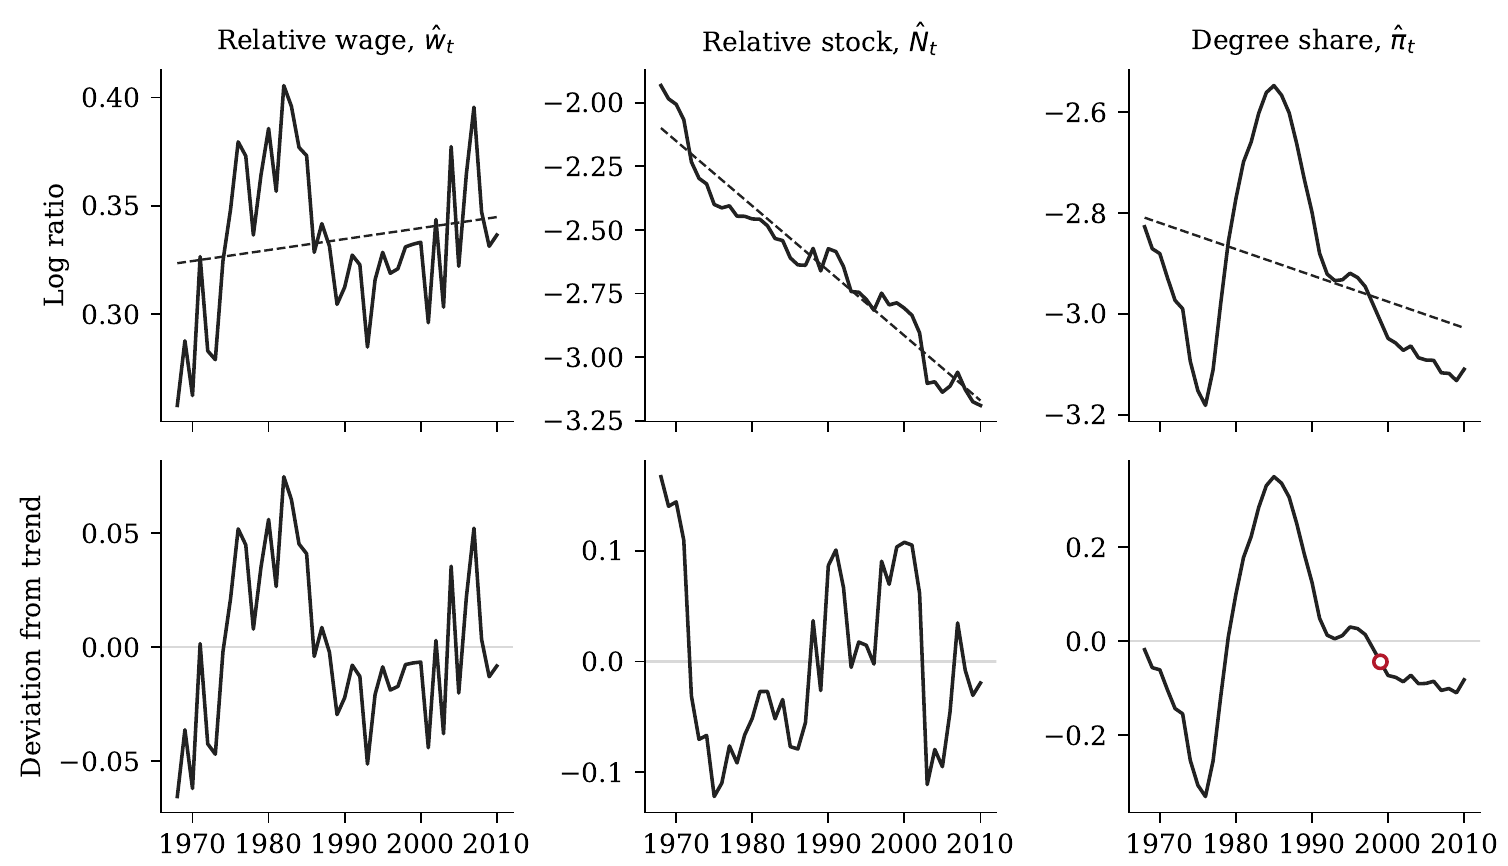
\includegraphics[width=\linewidth]{fig1.png}\end{minipage}
    \caption{Relative wage, stock, and degree share: log ratios (top), detrended (bottom)}
  \end{figure}
  \vspace{-0.3cm}
  \begin{itemize}\small
    \item \textbf{CPS ASEC (IPUMS):} median earnings and counts of engineers (OCC1990 044--059) vs.\ college graduates. \textbf{NSF:} bachelor's degrees by field.
    \item 43 observations; a \textbf{separate linear trend} removed from each series. Degree share: $-33$ log points (1976) to \alert{$+35$} (1985).
  \end{itemize}
\end{frame}

\begin{frame}{Estimation: Kalman-Filter Maximum Likelihood}
  \begin{itemize}
    \item \textbf{Observation equation} with serially correlated measurement error:
      \[ y_t=GX_t+v_t,\qquad v^x_{t+1}=D_xv^x_t+\sigma_xe^x_{t+1},\quad x\in\{w,N,\pi\},\; D_\pi=0. \]
    \item \textbf{Why:} only 611--1,409 engineers per CPS year; stock falls 17.7 log points in 2003 (new occupation codes); half the sample overlaps across years.
    \item State-space system $\Rightarrow$ Kalman filter $\Rightarrow$ \alert{exact Gaussian likelihood}:
      \[ \log L=\sum_{t=1}^T\Big[-\tfrac32\log2\pi-\tfrac12\log\det\Omega_t-\tfrac12a_t'\Omega_t^{-1}a_t\Big]. \]
    \item 14 parameters; Nelder--Mead $\to$ BFGS $\to$ Nelder--Mead; 7 of 8 starts agree.
    \item Likelihood is asymmetric $\Rightarrow$ \textbf{profile-likelihood} 95\% intervals: $LR(x)\le 3.84$.
  \end{itemize}
\end{frame}

% =====================================================
\section{Results}

\begin{frame}{Estimates: Demand, Enrollment, and Stock}
  \begin{table}
    \centering\footnotesize
    \begin{tabular}{llccc}
      \toprule
      & & & & Profile 95\% \\
      Parameter & Description & Estimate & S.E. & interval \\
      \midrule
      $f_2$ & Slope of inverse demand & 0.638 & (0.487) & [0.135, $>$6.32] \\
      $d$ & Enrollment cost slope & 0.075 & (0.054) & [$<$0.009, 0.439] \\
      $\lambda$ & Incumbents' share & 0.955 & (0.029) & [0.895, $>$0.995] \\
      \midrule
      $1/f_2$ & Demand elasticity & \alert{1.57} & (1.20) & \\
      $(1-\lambda)/d$ & Coefficient on $V_t$ & 0.59 & (0.38) & \\
      $\eta^{LR}$ & Long-run entry elasticity & \alert{6.07} & (3.63) & \\
      \bottomrule
    \end{tabular}
  \end{table}
  \begin{itemize}\small
    \item \textbf{Demand:} 1.57 lies within Ryoo--Rosen's 1.2--2.2; data rule out a nearly flat curve (elasticity $>7.4$), not a steep one.
    \item \textbf{Enrollment:} 6.07, above RR's 2.5--4.5, imprecise; data rule out \emph{insensitive} enrollment.
    \item \textbf{Stock:} $\lambda=0.955$ vs.\ accounting benchmark 0.959.
  \end{itemize}
\end{frame}

\begin{frame}{Shocks, Measurement Error, and Profile Likelihood}
  \begin{columns}[c]
    \begin{column}{0.52\textwidth}
      \begin{figure}
        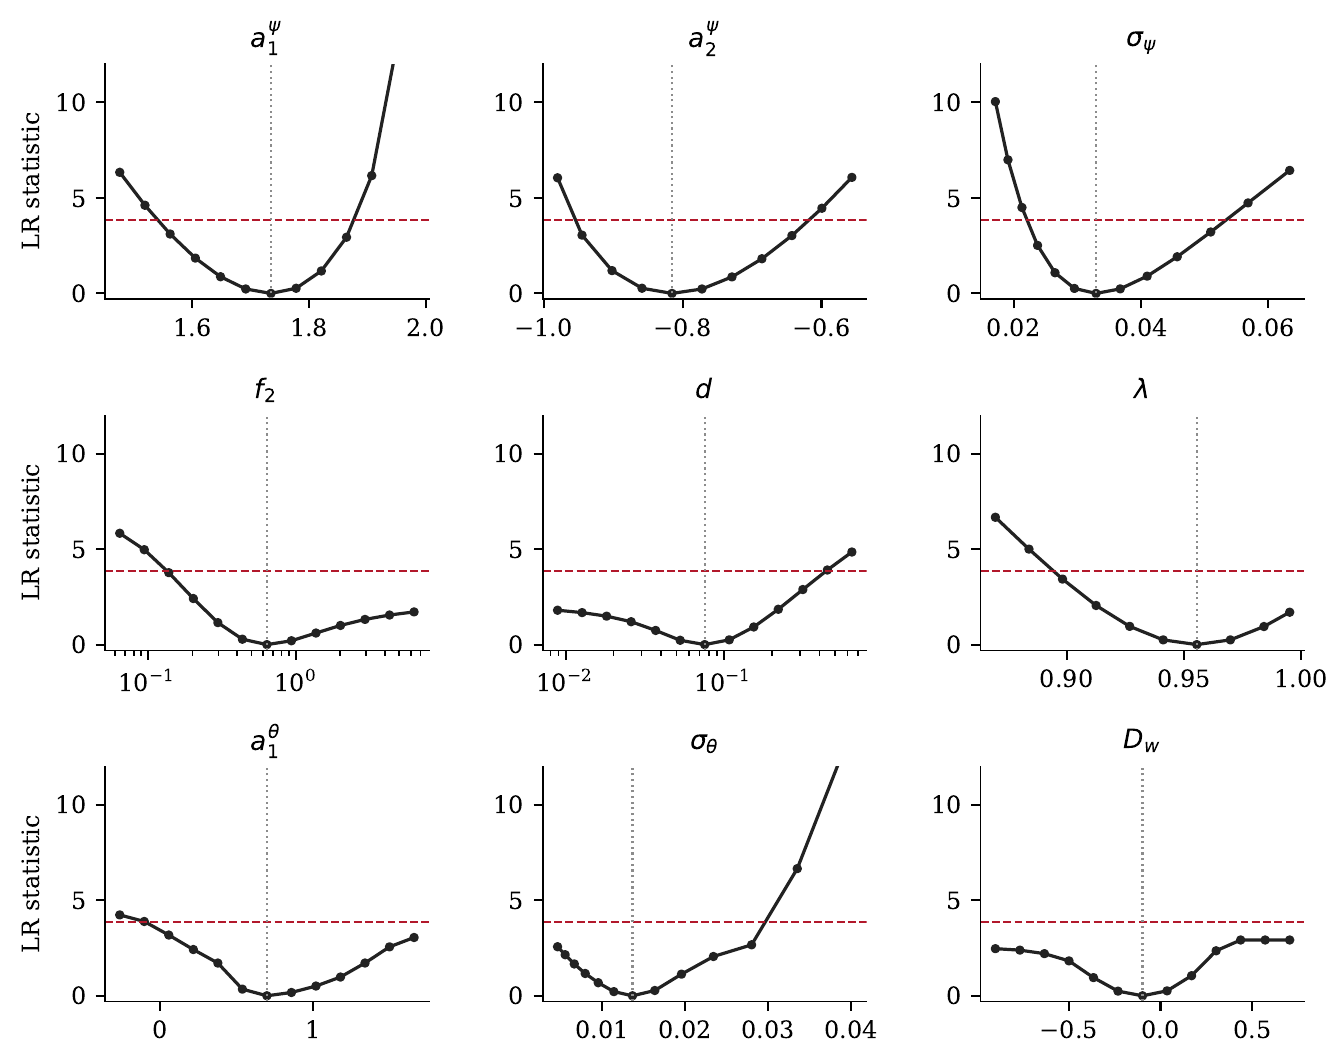
\includegraphics[width=\linewidth]{fig2.png}
        \caption{Profile likelihood $LR(x)$}
      \end{figure}
    \end{column}
    \begin{column}{0.46\textwidth}
      \begin{block}{Preference Shock $\psi$}
        \small
        Roots $0.867\pm0.251i$: modulus 0.90, \alert{period $\approx$ 22 years}. Real roots rejected: $LR=4.72>3.84$.
      \end{block}
      \vspace{0.15cm}
      \begin{block}{Demand Shock $\theta$}
        \small Real roots 0.89, $-0.20$; poorly determined.
      \end{block}
      \vspace{0.15cm}
      \begin{block}{Measurement Error}
        \small Stock error s.d.\ 0.049, persistence 0.73, vs.\ 0.079 for the stock itself: \alert{a noisy series}. Degree-share error at zero.
      \end{block}
    \end{column}
  \end{columns}
\end{frame}

\begin{frame}{Model Fit: Data vs.\ Simulated Moments}
  \begin{table}
    \centering\small
    \begin{tabular}{lcccc}
      \toprule
      & & \multicolumn{3}{c}{Model (1,000 samples)} \\
      \cmidrule(lr){3-5}
      & Data & Median & 5\% & 95\% \\
      \midrule
      \multicolumn{5}{l}{\textit{Standard deviation}} \\
      \quad $\tilde w_t$ & 0.035 & 0.028 & 0.021 & 0.040 \\
      \quad $\tilde N_t$ & 0.079 & 0.064 & 0.046 & 0.088 \\
      \quad $\tilde\pi_t$ & 0.169 & 0.118 & 0.065 & 0.195 \\
      \multicolumn{5}{l}{\textit{First-order autocorrelation}} \\
      \quad $\tilde w_t$ & 0.569 & 0.431 & 0.016 & 0.725 \\
      \quad $\tilde N_t$ & 0.765 & 0.657 & 0.408 & 0.816 \\
      \quad $\tilde\pi_t$ & 0.957 & 0.934 & 0.869 & 0.962 \\
      \multicolumn{5}{l}{\textit{Wage and future degree share}} \\
      \quad corr$(\tilde w_t,\tilde\pi_{t+4})$ & \alert{0.750} & 0.352 & $-0.118$ & 0.691 \\
      \quad corr$(\tilde w_t,\tilde\pi_{t+5})$ & \alert{0.763} & 0.365 & $-0.072$ & 0.711 \\
      \bottomrule
    \end{tabular}
  \end{table}
  \begin{itemize}\small
    \item Volatility and persistence: every data moment lies in the 5\%--95\% band.
    \item \textbf{The gap:} the wage--future degree correlation lies \alert{above the 95th percentile}.
  \end{itemize}
\end{frame}

% =====================================================
\section{Dynamics}

\begin{frame}{Impulse Responses}
  \begin{columns}[c]
    \begin{column}{0.54\textwidth}
      \begin{figure}
        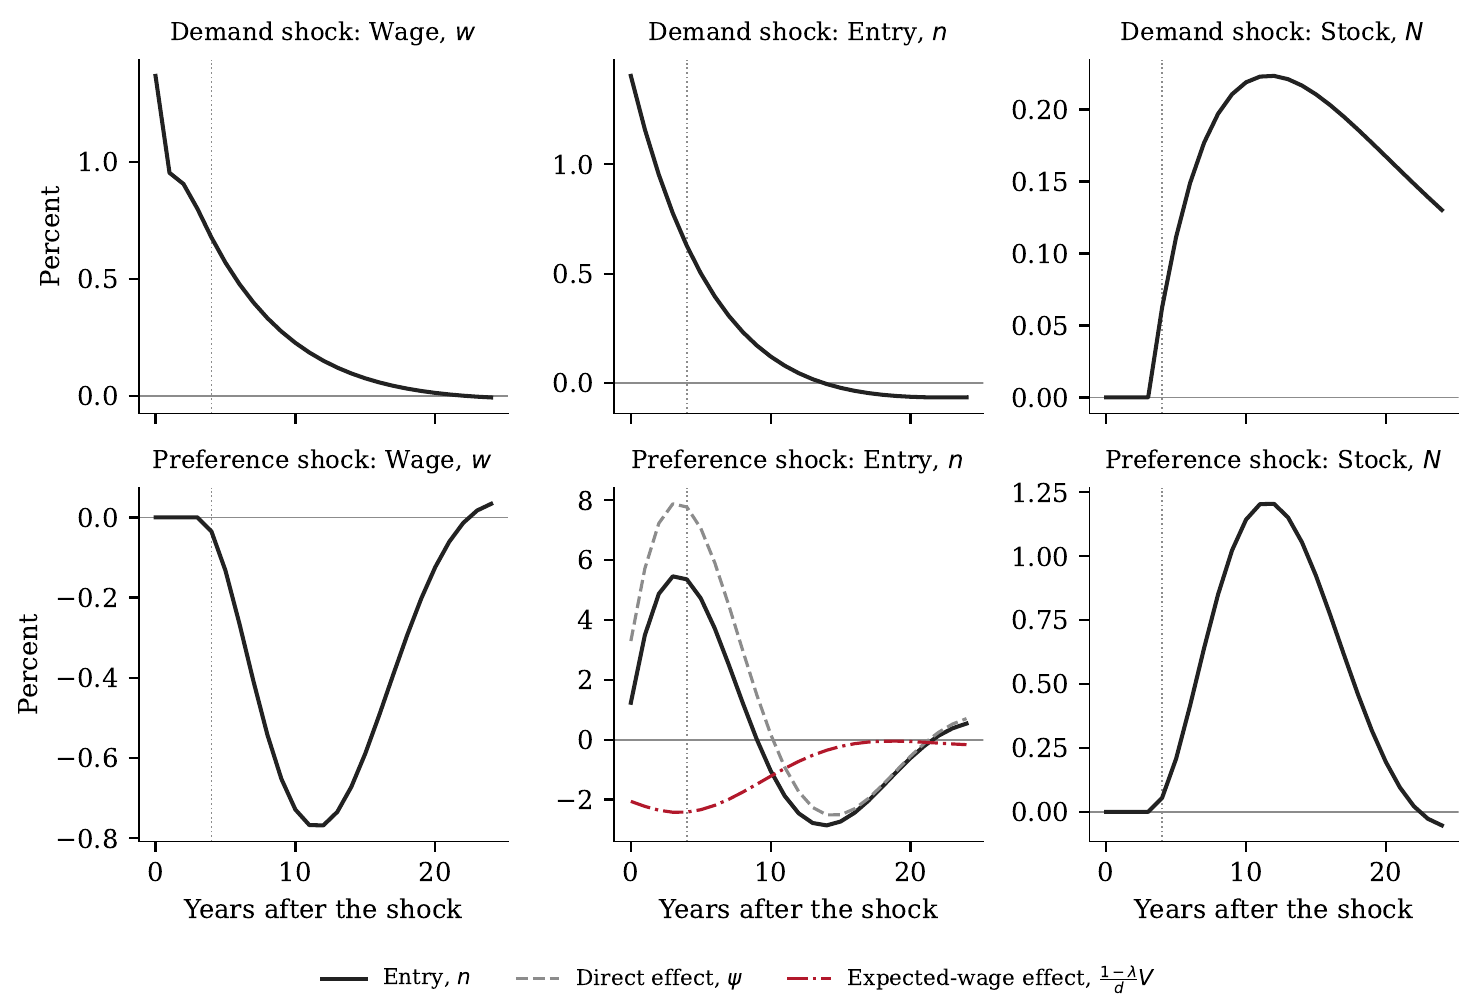
\includegraphics[width=\linewidth]{fig3.png}
        \caption{Demand (top) and preference (bottom) shocks}
      \end{figure}
    \end{column}
    \begin{column}{0.44\textwidth}
      \small
      \textbf{Demand shock:} students look through it.
      \begin{itemize}
        \item Wage $+1.37\%$, enrollment $+1.40\%$ at once.
        \item Wage gain halves in $\approx$ 4 years: $V_t$ rises 2.4 pts, not 14.0.
        \item Response $\approx$ \alert{1/6} of a permanent rise.
      \end{itemize}
      \vspace{0.15cm}
      \textbf{Preference shock:} largely self-offsetting.
      \begin{itemize}
        \item Enrollment rises \alert{37\%} of the shock.
        \item Foreseen glut lowers $V_t$, offsetting 63\%.
        \item Stock half-life: 15.2 years.
      \end{itemize}
    \end{column}
  \end{columns}
\end{frame}

\begin{frame}{Variance Decomposition}
  \begin{table}
    \centering\small
    \begin{tabular}{lccc|ccc}
      \toprule
      & \multicolumn{3}{c|}{Observed series} & \multicolumn{3}{c}{Model variables} \\
      & $\tilde w_t$ & $\tilde N_t$ & $\tilde\pi_t$ & $w_t$ & $N_t$ & $n_t$ \\
      \midrule
      Demand shock & 0.42 & 0.01 & 0.03 & 0.56 & 0.07 & 0.03 \\
      Preference shock & 0.34 & 0.18 & \alert{0.97} & 0.44 & 0.93 & \alert{0.97} \\
      Measurement error & 0.24 & \alert{0.81} & 0.00 & & & \\
      \bottomrule
    \end{tabular}
  \end{table}
  \vspace{0.2cm}
  \begin{enumerate}
    \item \textbf{97\%} of the variance of enrollment and the degree share comes from the \alert{preference shock}: swings in the choice of major reflect the attractiveness of engineering, not wages.
    \item \textbf{81\%} of the variance of the observed stock is \alert{measurement error}.
    \item Both shocks matter for wages: demand 56\%, preference 44\% of the true wage's variance.
  \end{enumerate}
\end{frame}

% =====================================================
\section[RE vs.\ Cobweb]{Rational Expectations versus the Cobweb}

\begin{frame}{Rational Expectations versus the Cobweb}
  \begin{table}
    \centering\small
    \begin{tabular}{lcc}
      \toprule
      & Rational expectations & Cobweb \\
      \midrule
      $\log L$ & 260.47 & 262.00 \\
      $\lambda$ & 0.955 & 0.946 \\
      Entry elasticity ($\eta^{LR}$ / $\eta$) & 6.07 & 5.10 \\
      \alert{Demand elasticity $1/f_2$} & \alert{1.57} & \alert{5.99} \\
      Demand shock: modulus, period & 0.89, real roots & 0.97, 25.5 yr \\
      Demand innovation s.d.\ $\sigma_\theta$ & 0.0137 & 0.0019 \\
      Preference shock: modulus, period & 0.90, 22.3 yr & 0.86, 16.4 yr \\
      \bottomrule
    \end{tabular}
  \end{table}
  \begin{itemize}\small
    \item Same data and likelihood; 14 parameters each, not nested: a 1.5 gap in $\log L$ \textbf{does not discriminate}.
    \item Agreement on $\lambda$, stock noise, and a \textbf{strong entry response}.
    \item Differences on the \textbf{demand side}: a nearly flat curve and an almost deterministic long demand cycle.
  \end{itemize}
\end{frame}

\begin{frame}{The Cobweb Matches the Wage--Degree Link}
  \begin{figure}
    \centering
    \begin{minipage}{0.74\linewidth}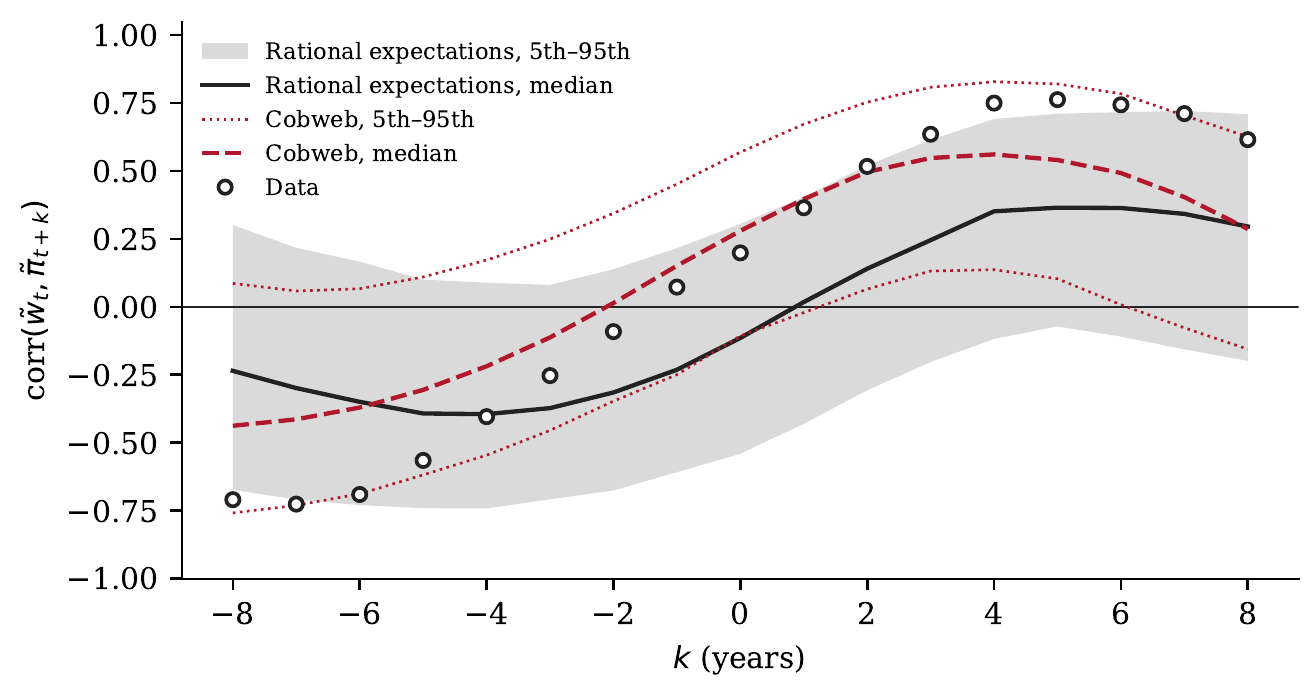
\includegraphics[width=\linewidth]{fig4.png}\end{minipage}
    \caption{Correlation of the wage with the degree share $k$ years later}
  \end{figure}
  \vspace{-0.2cm}
  \begin{itemize}\small
    \item At $k=4$: data \alert{0.75}; RE median 0.35, band $[-0.12, 0.69]$; cobweb median 0.56, band $[0.14, 0.83]$ \textbf{covers the data}.
    \item Cobweb students treat today's wage as permanent: a 1\% wage rise raises enrollment \alert{5.1\%} on impact vs.\ $\approx$ 1.0\% under RE.
  \end{itemize}
\end{frame}

\begin{frame}{Responses under the Two Forms of Expectations}
  \begin{figure}
    \centering
    \begin{minipage}{0.62\linewidth}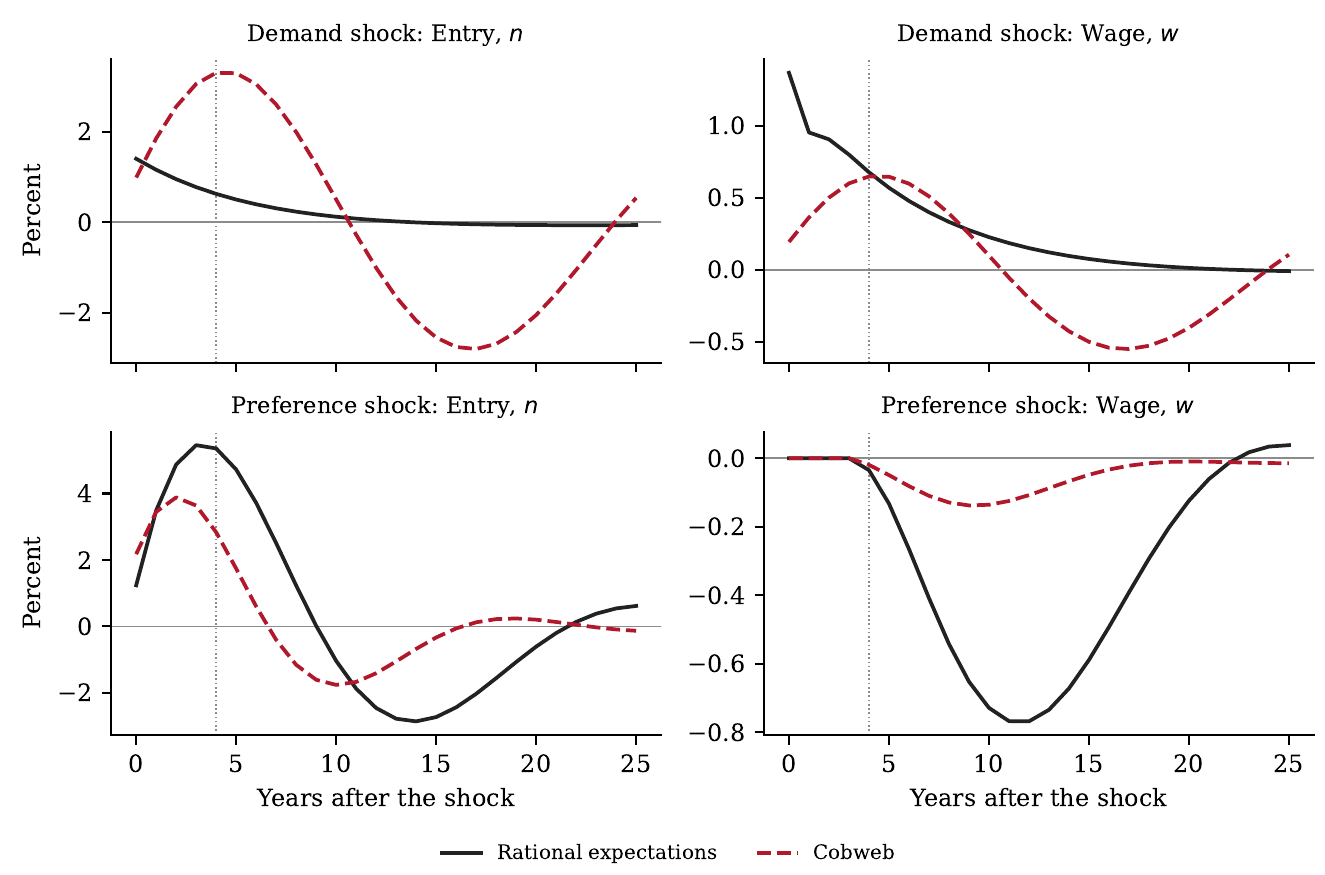
\includegraphics[width=\linewidth]{fig5.png}\end{minipage}
    \caption{Solid: rational expectations; dashed: cobweb}
  \end{figure}
  \vspace{-0.2cm}
  \begin{itemize}\small
    \item \textbf{Demand shock:} the classic cobweb cycle --- high wage, entry surge, glut four years later, wage falls, entry below normal (partly from the demand cycle itself).
    \item \textbf{Preference shock:} cobweb enrollment moves one for one for four years; under RE it rises only 37\% on impact.
  \end{itemize}
\end{frame}

% =====================================================
\section{Conclusion}

\begin{frame}{Conclusion}
  \begin{block}{Summary}
    Enrollment responds \textbf{strongly to persistent} wage changes, yet the large swings in degrees come mainly ($\approx$ 97\%) from the \alert{attractiveness of engineering}. Whether students look through temporary wages, the data cannot tell --- so the \alert{demand elasticity} depends on expectations (1.6 vs.\ 6.0).
  \end{block}
  \vspace{0.2cm}
  \begin{itemize}\small
    \item \textbf{Limitations:} $\beta$ fixed at 0.96; linear detrending; independent shocks; no enrollment adjustment costs; only 43 observations; 81\% of stock variance is measurement error.
    \item \textbf{Extensions:} physicians, lawyers, teachers, scientists --- same planning problem, state space, and likelihood, with the state vector adjusted to the length of training.
  \end{itemize}
  \vspace{0.3cm}
  \begin{center}
    \Large\textcolor{pkured}{Thank you!}
  \end{center}
\end{frame}


% =====================================================
%                    APPENDIX
% =====================================================
\appendix
\setbeamertemplate{footline}{%
  \hfill\usebeamercolor[fg]{normal text}\scriptsize Appendix\,--\,\insertframenumber\hspace*{3mm}\vspace*{2.5mm}}

\section{Derivations}

\begin{frame}{Appendix A.1: Stock Accumulation}
  \small
  \begin{itemize}
    \item Divide $L_{t+1}=\delta L_t+S_{t-3}$ by $L_t$. On a balanced growth path, $L_{t+1}/L_t=1+g$ and $S_{t-3}/L_t=\bar s$, so
      \[ 1+g=\delta+\bar s . \]
    \item Let $\hat\ell_t,\hat s_t$ be log deviations of $L_t,S_t$ from the path. A first-order expansion of
      \[ (1+g)\,e^{\hat\ell_{t+1}-\hat\ell_t}=\delta+\bar s\,e^{\hat s_{t-3}-\hat\ell_t} \]
      gives
      \[ (1+g)(\hat\ell_{t+1}-\hat\ell_t)=\bar s\,(\hat s_{t-3}-\hat\ell_t)
         \;\Longrightarrow\;
         \hat\ell_{t+1}=\lambda\hat\ell_t+(1-\lambda)\hat s_{t-3}, \]
      with $\lambda=\delta/(1+g)$ and $1-\lambda=\bar s/(1+g)$.
    \item Subtract the same equation for all college graduates (superscript $c$), with $N_t=\hat\ell_t-\hat\ell^c_t$, $n_t=\hat s_t-\hat s^c_t$:
      \[ N_{t+1}=\lambda N_t+(1-\lambda)n_{t-3}+\underbrace{(\lambda-\lambda^c)\big(\hat\ell^c_t-\hat s^c_{t-3}\big)}_{\text{dropped}} . \]
    \item In the data the last term has detrended s.d.\ \alert{0.0022}, against 0.0787 for $N_t$.
  \end{itemize}
\end{frame}

\begin{frame}{Appendix A.2: Household First-Order Condition}
  \footnotesize
  \begin{itemize}
    \item Iterating the constraint $N^h_{t+1}=\lambda N^h_t+(1-\lambda)n_{t-3}$:
      \[ \frac{\partial N^h_s}{\partial n_t}=(1-\lambda)\lambda^{\,s-t-4}\quad (s\ge t+4),\qquad 0\ \text{otherwise}. \]
    \item Taking wages as given, the derivative of the objective w.r.t.\ $n_t$, divided by $\beta^t$:
      \[ -d\,(n_t-\psi_t)+(1-\lambda)\,\E_t\sum_{j=0}^\infty\beta^{4+j}\lambda^j w_{t+4+j}=0,
         \qquad \text{second derivative } -d<0 . \]
      Rearranging: $n_t=\frac{1-\lambda}{d}V_t+\psi_t$ with $V_t=\beta^4\E_t\sum_j(\beta\lambda)^jw_{t+4+j}$.
    \item \textbf{Long-run elasticity.} If $w_{t+k}$ rises by one unit for all $k\ge0$:
      \[ \Delta V_t=\beta^4\sum_{j\ge0}(\beta\lambda)^j=\frac{\beta^4}{1-\beta\lambda}=10.26,
         \qquad \Delta n_t=\eta^{LR}=\tfrac{1-\lambda}{d}\times10.26\approx6.07 . \]
    \item \textbf{Cobweb.} $\E_tw_{t+j}=w_t\Rightarrow V_t=\frac{\beta^4w_t}{1-\beta\lambda}\Rightarrow n_t=\eta w_t+\psi_t$. Using $w_t=-f_2N_t+\theta_t$:
      \[ n_t=-\eta f_2N_t+\eta\theta_t+\psi_t\equiv KX_t,\quad X_{t+1}=(A+BK)X_t+C\varepsilon_{t+1}. \]
  \end{itemize}
\end{frame}

\begin{frame}{Appendix A.3: AR(2) Processes with Complex Roots}
  \small
  \begin{itemize}
    \item The impulse response $x_h=\partial x_{t+h}/\partial\varepsilon_t$ of $x_t=a_1x_{t-1}+a_2x_{t-2}+\varepsilon_t$ solves
      \[ x_h=a_1x_{h-1}+a_2x_{h-2},\qquad x_0=1,\; x_{-1}=0 . \]
    \item With distinct roots $z_{1,2}$ of $z^2=a_1z+a_2$:\quad $x_h=\dfrac{z_1^{h+1}-z_2^{h+1}}{z_1-z_2}$.
    \item If $a_1^2+4a_2<0$: $z_{1,2}=re^{\pm i\omega}$ with $r^2=z_1z_2=-a_2$ and $r\cos\omega=a_1/2$, so
      \[ x_h=\frac{2i\,r^{h+1}\sin\big((h+1)\omega\big)}{2i\,r\sin\omega}
            =r^h\,\frac{\sin\big((h+1)\omega\big)}{\sin\omega}, \]
      an oscillation with period $2\pi/\omega$ whose amplitude decays at rate $r$.
  \end{itemize}
  \begin{block}{Application to the Preference Shock}
    $a_1^\psi=1.735$, $a_2^\psi=-0.815$: $r=\sqrt{0.815}=0.90$, $\cos\omega=1.735/(2\times0.90)$ $\Rightarrow$ period $2\pi/\omega\approx22.3$ years.\\[0.5ex]
    Test of real roots, $H_0:(a_1^\psi)^2+4a_2^\psi\ge0$: $LR=4.72$. At the least favorable boundary point the statistic is $\tfrac12\chi^2_0+\tfrac12\chi^2_1$ (5\% critical value 2.71) $\Rightarrow$ \alert{rejected}.
  \end{block}
\end{frame}

\begin{frame}{Appendix A.4: Proof of Proposition 1}
  \small
  \begin{itemize}
    \item Since $\partial\big(\theta_sN_s-\tfrac{f_2}{2}N_s^2\big)/\partial N_s=\theta_s-f_2N_s$, the planner's first-order condition for $n_t$ is
      \[ d\,(n_t-\psi_t)=(1-\lambda)\,\E_t\sum_{j=0}^\infty\beta^{4+j}\lambda^j\big(\theta_{t+4+j}-f_2N_{t+4+j}\big). \tag{$\ast$} \]
    \item For $f_2,d>0$ the objective is strictly concave and the constraints linear; for processes with bounded second moments, $\beta<1$ ensures transversality. Hence $\{N_t,n_t\}$ solves the planning problem \textbf{iff} $(\ast)$ holds for all $t$, and the solution is unique.
    \item \textbf{Necessity.} In an equilibrium, substitute the firm's condition $w_s=\theta_s-f_2N_s$ into the household's condition $\Rightarrow(\ast)$.
    \item \textbf{Sufficiency.} Let $\{N_t,n_t\}$ satisfy $(\ast)$; set $w_s=\theta_s-f_2N_s$ and $N^d_s=N^h_s=N_s$. Then the demand curve and market clearing hold by construction, and $(\ast)$ becomes the household's condition. Both private problems are strictly concave, so these first-order conditions are sufficient: the allocation with this wage is an equilibrium.
    \item \textbf{Uniqueness} follows from that of the planner's solution. \hfill$\square$
  \end{itemize}
\end{frame}

\begin{frame}{Appendix A.5: Linear-Quadratic Representation}
  \footnotesize
  $X_t=(N_t,\,n_{t-1},\,n_{t-2},\,n_{t-3},\,n_{t-4},\,\theta_t,\,\psi_t,\,\theta_{t-1},\,\psi_{t-1})'$,\quad $u_t=n_t$,\quad
  $X_{t+1}=AX_t+Bu_t+C\varepsilon_{t+1}$:
  \[
  \setlength{\arraycolsep}{2.6pt}
  A=\begin{pmatrix}
    \lambda&0&0&1-\lambda&0&0&0&0&0\\
    0&0&0&0&0&0&0&0&0\\
    0&1&0&0&0&0&0&0&0\\
    0&0&1&0&0&0&0&0&0\\
    0&0&0&1&0&0&0&0&0\\
    0&0&0&0&0&a_1^\theta&0&a_2^\theta&0\\
    0&0&0&0&0&0&a_1^\psi&0&a_2^\psi\\
    0&0&0&0&0&1&0&0&0\\
    0&0&0&0&0&0&1&0&0
  \end{pmatrix},\quad
  B=\begin{pmatrix}0\\1\\0\\0\\0\\0\\0\\0\\0\end{pmatrix},\quad
  C=\begin{pmatrix}0&0\\0&0\\0&0\\0&0\\0&0\\\sigma_\theta&0\\0&\sigma_\psi\\0&0\\0&0\end{pmatrix}.
  \]
  \begin{itemize}
    \item Period return $r(X_t,u_t)=X_t'RX_t+Qu_t^2+2u_tWX_t$, where the only nonzero elements of $R$ are $R_{11}=-f_2/2$ and $R_{16}=R_{61}=1/2$; $Q=-d/2$; and $W$ has $d/2$ in the position of $\psi_t$, zeros elsewhere.
    \item These reproduce $\theta_tN_t-\tfrac{f_2}{2}N_t^2-\tfrac d2n_t^2+d\,\psi_tn_t$.
  \end{itemize}
\end{frame}

\begin{frame}{Appendix A.6: Solving the Planning Problem}
  \small
  \begin{itemize}
    \item Quadratic value function $v(X)=X'PX+c$; Bellman equation:
      \begin{align*} X'PX+c=\max_u\Big\{&X'RX+Qu^2+2uWX\\ &+\beta(AX+Bu)'P(AX+Bu)+\beta\,\mathrm{tr}(C'PC)+\beta c\Big\}. \end{align*}
    \item First-order condition $\Rightarrow$ decision rule
      \[ u_t=-FX_t,\qquad F=(Q+\beta B'PB)^{-1}(W+\beta B'PA). \]
    \item Matching quadratic terms $\Rightarrow$ algebraic Riccati equation
      \[ P=R+\beta A'PA-(W'+\beta A'PB)(Q+\beta B'PB)^{-1}(W+\beta B'PA). \]
    \item \textbf{Second-order condition:} $B$ selects only $n_{t-1}$, so $Q+\beta B'PB\le-d/2<0$. $F$ does not depend on $C$: \alert{certainty equivalence}. Solved after rescaling $(A,B)$ by $\sqrt\beta$.
    \item Law of motion $X_{t+1}=MX_t+C\varepsilon_{t+1}$, $M=A-BF$; since $\E_tX_{t+k}=M^kX_t$,
      \[ V_t=\beta^4\sum_{j\ge0}(\beta\lambda)^jG_wM^{4+j}X_t=\beta^4G_wM^4(I-\beta\lambda M)^{-1}X_t . \]
  \end{itemize}
\end{frame}

\section{Likelihood}

\begin{frame}{Appendix B.1: State-Space System and Kalman Filter}
  \small
  \begin{itemize}
    \item $s_t=(X_t',v_t')'$, $\epsilon_t=(\varepsilon^\theta_t,\varepsilon^\psi_t,e^w_t,e^N_t,e^\pi_t)'\sim\text{i.i.d. }N(0,I_5)$:
      \[ s_{t+1}=\mathcal Ms_t+\mathcal C\epsilon_{t+1},\qquad y_t=\mathcal Gs_t, \]
      \[ \mathcal M=\begin{pmatrix}M&0\\0&D\end{pmatrix},\;
         \mathcal C=\begin{pmatrix}C&0\\0&\Sigma_v\end{pmatrix},\;
         \mathcal G=\begin{pmatrix}G&I_3\end{pmatrix}, \]
      $D=\mathrm{diag}(D_w,D_N,0)$, $\Sigma_v=\mathrm{diag}(\sigma_w,\sigma_N,\sigma_\pi)$; rows of $G$ select $w_t=-f_2N_t+\theta_t$, $N_t$, $\pi_t=n_{t-4}$.
    \item Let $\hat s_t=E[s_t\mid y^{t-1}]$, $\Sigma_t=\mathrm{Var}(s_t\mid y^{t-1})$, started at the stationary distribution $\hat s_1=0$, $\Sigma_1=\mathcal M\Sigma_1\mathcal M'+\mathcal C\mathcal C'$.
    \item Joint normality of $(s_{t+1},y_t)\mid y^{t-1}$ gives the recursions:
      \begin{align*}
        a_t&=y_t-\mathcal G\hat s_t, & \Omega_t&=\mathcal G\Sigma_t\mathcal G',\\
        K_t&=\mathcal M\Sigma_t\mathcal G'\Omega_t^{-1}, & \hat s_{t+1}&=\mathcal M\hat s_t+K_ta_t,\\
        \Sigma_{t+1}&=(\mathcal M-K_t\mathcal G)\Sigma_t(\mathcal M-K_t\mathcal G)'+\mathcal C\mathcal C'. &&
      \end{align*}
    \item The last form is a sum of positive semidefinite matrices (numerically stable).
  \end{itemize}
\end{frame}

\begin{frame}{Appendix B.2: Likelihood, Moments, and Optimization}
  \small
  \begin{itemize}
    \item \textbf{Prediction-error decomposition.} For $r<t$, $a_r$ is a function of $y^{t-1}$ and $E[a_t\mid y^{t-1}]=0$, so $E[a_ta_r']=0$; being normal, innovations are independent. The map $y^T\mapsto a^T$ is triangular with unit Jacobian:
      \[ f(y_1,\dots,y_T)=\prod_{t=1}^T(2\pi)^{-3/2}\det(\Omega_t)^{-1/2}\exp\!\Big(-\tfrac12a_t'\Omega_t^{-1}a_t\Big). \]
    \item \textbf{Population moments.} $\Sigma=\mathcal M\Sigma\mathcal M'+\mathcal C\mathcal C'$; autocovariances $\Gamma_k=\mathcal G\mathcal M^k\Sigma\mathcal G'$.
    \item \textbf{Variance decomposition.} Shocks are independent, so $\Sigma=\sum_j\Sigma^{(j)}$ with $\Sigma^{(j)}=\mathcal M\Sigma^{(j)}\mathcal M'+\mathcal C_j\mathcal C_j'$; share of shock $j$ in series $i$: $[\mathcal G\Sigma^{(j)}\mathcal G']_{ii}/[\mathcal G\Sigma\mathcal G']_{ii}$.
    \item \textbf{Reparametrization.} $f_2,d,\sigma$'s $=\exp(\cdot)$; $\lambda$ logistic; $a_2,D_w,D_N=\tanh(\cdot)$; $a_1=(1-a_2)\tanh(z)$ keeps each AR(2) stationary. If the Riccati equation fails, $M$ is unstable, or some $\Omega_t\not\succ0$: $\log L=-10^{10}$.
  \end{itemize}
\end{frame}

\section{References}

\setbeamertemplate{bibliography item}{}
\setbeamercolor{bibliography entry author}{fg=black}
\setbeamercolor{bibliography entry title}{fg=black}
\setbeamercolor{bibliography entry location}{fg=black!70}
\setbeamercolor{bibliography entry note}{fg=black!70}

\begin{frame}[allowframebreaks]{References}
  \scriptsize
  \begin{thebibliography}{99}
    \bibitem{altug} Altug, S. (1989). Time-to-build and aggregate fluctuations: Some new evidence. \emph{International Economic Review}, 30(4), 889--920.
    \bibitem{arrow} Arrow, K. J. \& Capron, W. M. (1959). Dynamic shortages and price rises: The engineer-scientist case. \emph{Quarterly Journal of Economics}, 73(2), 292--308.
    \bibitem{ipums} Flood, S., King, M., Rodgers, R., Ruggles, S., Warren, J. R., et al.\ (2025). IPUMS CPS: Version 13.0 [dataset]. Minneapolis, MN: IPUMS. \texttt{doi:10.18128/D030.V13.0}.
    \bibitem{freeman71} Freeman, R. B. (1971). \emph{The Market for College-Trained Manpower: A Study in the Economics of Career Choice}. Harvard University Press.
    \bibitem{freeman75} Freeman, R. B. (1975). Supply and salary adjustments to the changing science manpower market: Physics, 1948--1973. \emph{American Economic Review}, 65(1), 27--39.
    \bibitem{freeman76} Freeman, R. B. (1976). A cobweb model of the supply and starting salary of new engineers. \emph{Industrial and Labor Relations Review}, 29(2), 236--248.
    \bibitem{hall} Hall, G. J. (1996). Overtime, effort, and the propagation of business cycle shocks. \emph{Journal of Monetary Economics}, 38(1), 139--160.
    \bibitem{hs80} Hansen, L. P. \& Sargent, T. J. (1980). Formulating and estimating dynamic linear rational expectations models. \emph{Journal of Economic Dynamics and Control}, 2, 7--46.
    \bibitem{hs13} Hansen, L. P. \& Sargent, T. J. (2013). \emph{Recursive Models of Dynamic Linear Economies}. Princeton University Press.
    \bibitem{ireland} Ireland, P. N. (2004). A method for taking models to the data. \emph{Journal of Economic Dynamics and Control}, 28(6), 1205--1226.
    \bibitem{nsf} National Science Foundation, National Center for Science and Engineering Statistics (2013). Science and engineering degrees: 1966--2010. Detailed Statistical Tables NSF 13-327.
    \bibitem{rr} Ryoo, J. \& Rosen, S. (2004). The engineering labor market. \emph{Journal of Political Economy}, 112(S1), S110--S140.
    \bibitem{sargent78} Sargent, T. J. (1978). Estimation of dynamic labor demand schedules under rational expectations. \emph{Journal of Political Economy}, 86(6), 1009--1044.
    \bibitem{sargent89} Sargent, T. J. (1989). Two models of measurements and the investment accelerator. \emph{Journal of Political Economy}, 97(2), 251--287.
    \bibitem{siow} Siow, A. (1984). Occupational choice under uncertainty. \emph{Econometrica}, 52(3), 631--646.
    \bibitem{bls} U.S. Bureau of Labor Statistics (n.d.). Occupation and industry classification systems used in the Current Population Survey. \texttt{bls.gov/cps/cpsoccind.htm}.
    \bibitem{zarkin} Zarkin, G. A. (1985). Occupational choice: An application to the market for public school teachers. \emph{Quarterly Journal of Economics}, 100(2), 409--446.
  \end{thebibliography}
\end{frame}

\end{document}
